\documentclass[]{elsarticle} %review=doublespace preprint=single 5p=2 column
%%% Begin My package additions %%%%%%%%%%%%%%%%%%%
\usepackage[hyphens]{url}

  \journal{Forest Ecology and Management} % Sets Journal name


\usepackage{lineno} % add
\providecommand{\tightlist}{%
  \setlength{\itemsep}{0pt}\setlength{\parskip}{0pt}}

\usepackage{graphicx}
\usepackage{booktabs} % book-quality tables
%%%%%%%%%%%%%%%% end my additions to header

\usepackage[T1]{fontenc}
\usepackage{lmodern}
\usepackage{amssymb,amsmath}
\usepackage{ifxetex,ifluatex}
\usepackage{fixltx2e} % provides \textsubscript
% use upquote if available, for straight quotes in verbatim environments
\IfFileExists{upquote.sty}{\usepackage{upquote}}{}
\ifnum 0\ifxetex 1\fi\ifluatex 1\fi=0 % if pdftex
  \usepackage[utf8]{inputenc}
\else % if luatex or xelatex
  \usepackage{fontspec}
  \ifxetex
    \usepackage{xltxtra,xunicode}
  \fi
  \defaultfontfeatures{Mapping=tex-text,Scale=MatchLowercase}
  \newcommand{\euro}{€}
\fi
% use microtype if available
\IfFileExists{microtype.sty}{\usepackage{microtype}}{}
\bibliographystyle{elsarticle-harv}
\usepackage{longtable}
\usepackage{graphicx}
% We will generate all images so they have a width \maxwidth. This means
% that they will get their normal width if they fit onto the page, but
% are scaled down if they would overflow the margins.
\makeatletter
\def\maxwidth{\ifdim\Gin@nat@width>\linewidth\linewidth
\else\Gin@nat@width\fi}
\makeatother
\let\Oldincludegraphics\includegraphics
\renewcommand{\includegraphics}[1]{\Oldincludegraphics[width=\maxwidth]{#1}}
\ifxetex
  \usepackage[setpagesize=false, % page size defined by xetex
              unicode=false, % unicode breaks when used with xetex
              xetex]{hyperref}
\else
  \usepackage[unicode=true]{hyperref}
\fi
\hypersetup{breaklinks=true,
            bookmarks=true,
            pdfauthor={},
            pdftitle={Effects of forest management and harvest intensity on landscape level wind damage risk},
            colorlinks=false,
            urlcolor=blue,
            linkcolor=magenta,
            pdfborder={0 0 0}}
\urlstyle{same}  % don't use monospace font for urls

\setcounter{secnumdepth}{5}
% Pandoc toggle for numbering sections (defaults to be off)


% Pandoc header



\begin{document}
\begin{frontmatter}

  \title{Effects of forest management and harvest intensity on landscape level wind damage risk}
    \author[Department of Biological and Environmental Science]{Mária Potterf\corref{1}}
   \ead{mpotterf@jyu.fi} 
    \author[Department of Biological and Environmental Science]{Kyle Eyvindson}
   \ead{kyle.j.eyvindson@jyu.fi} 
    \author[Department of Biological and Environmental Science]{Clemens Blattert}
   \ead{clemens.c.blattert@jyu.fi} 
    \author[Department of Biological and Environmental Science]{Daniel Burgas}
   \ead{daniel.d.burgas-riera@jyu.fi} 
    \author[Department of Biological and Environmental Science]{Mikko Mönkkönen}
   \ead{mikko.monkkonen@jyu.fi} 
      \address[University of Jyvaskyla]{Department of Biological and Environmental Science, University of Jyvaskyla, P.O. Box 35, FI-40014 Jyvaskyla, Finland}
    \address[Wisdom]{This is wisdom address}
    \address[LUKE]{THIS is Luke address Department, Street, City, State, Zip}
      \cortext[1]{Corresponding Author}
    \cortext[]{}
  
  \begin{abstract}
  Future forest management needs to balance between simultaneous provision of timber, supporting non-woody ecosystem services, and shelter biodiversity. New techniques to atteint this goal emerge: landscape-level optimization of forest managements, increasing proportion of set-aside forest stands, and new harvesting techniques, such as continuous forest cover. Yet, novel stand- and landscape-level management shape forest structures and define future stand vulnerability to more frequent climatic disruptions, such as windthrows under hardening climate change.
  To understand how will the traditional (rotation forestry, RF) and novel forest managements techniques (continuous cover forest, CCF) combined by optimal management alternate the probability of wind risk, we simulated forest stand dynamics under groups of alternative management regimes (RF, CCF and combined: ALL) optimized over the range of harvesting intensity gradient to calculate stand level probability of wind damage over 100 years period. We further investigate the effects of wind damage risk by the pulp and log timber volume at risk under variaous scenarios and over time.
  We found that stands under CCF have higher wind risk probability than RF, and RF maintains levels of wind risk over time, while in CCF risk increases. Yet, the pulp timber at risk under RF is three times higher then in CCF under all harvest intensities. The CCF dominates in production of log wood, whereas pulp wood in intensive harvesting (RF) creates up to 1/2 of the total standing volume. RF produces smaller, younger trees (15 m and mean age of 50) compared to CCF (22m and 80 years) (!!! WHAT ID DBH???), and maintains less trees over stand. The stands under SA regimes have similar trends over harvest intensity level and time, independent of prevailing regimes applied over landscapes. We conclude that althought CCF increases landscape level wind risk, it equalizes the exposed timber volume at risk over time, compared to RF that culminates volume at risk to certain time - right beforet the harvest.\\
  \end{abstract}
  
 \end{frontmatter}

\newpage

\hypertarget{introduction}{%
\section{Introduction}\label{introduction}}

Clarify tha main question of the manuscripts: how will the future

Future forest ecosystems should simultaneously deliver timber, non-woody ecosystem services and shelter biodiversity under increasing rates of future forest disturbances.

Future forest ecosystems need to simultaneously provide timber, non-woody ecosystem services such as carbon storage or human recreation, and shelter biodiversity.\\
To balance between biodiversity and timber economic gains, the proportion of set-aside forests within commercial forests emerges, and new forest management approaches are explored, such as continuous forest cover (Eyvindson et al., 2021) and traditional harvesting regimes are becoming controversial or requested to ban (\ldots{}). The increase of the set aside forests within the commercial forests, as well as development of the new management techniques affect landscape level structural diversity, timing of the thinning, presence of absence of the final cuts in rotation forestry or development of the larger trees within continuous cover forestry or in set-aside forestry. The fundamental is the carefull landscape level planning of the management actions balancing between set-aside (unmanaged forests), intensive management and continuously present forest cover.

Optimal management scenarios fullfil the specific objectives of the society of forest owners to provide certain timber value, improve provision of timber and non-timber ecosystem services, or improve overall forest multifunctionality of the landscape. As such, optimization provides the combination of the specific forest management regimes on stand level. Althought the optimization process does not necessary involve the spatial configuration of the stands, it specifically assigns the particular regimes to individual stands and therefore allows to recreate alternative dynamics landscapes shaped by forest managements aggregated by optimal scenarios. As such, the spatial configuration of the management regimes allows to estimate the subsequent characteristics such as landscape level risk of wind damage.

The risk of the wind damage increases with current climate change and it creates the major risk to the stability of the forest production. Windthrows are unpredictable climatic disruption that shapes forest structure and composition, and if left unsalvaged could create opportiunities for deadwood dependent species and support local biodiversity. From economical point of view, however, windthrows massively abrupt the continuity of the timber supply, lowers timber quality from log to pulp, increases the prices of unplanned salvage harvesting (REF). To lower the risk of wind risk damage, current suggestions include shortening the rotation period, promoting/avoiding the wind resistant vs.~wind prone tree specuies, advocate for shortening of the minimal stand age (Latvia REF). This however poses further pressure on the multifucntionnal and multiple objective oriented landscapes, which will provide habitats for endangered species, support non-timber services and forest recreational use.

Traditional forest management regimes specialized in promoting timber revenues while minimizing costs. In Fennoscandia, over the decades, the traditional rotation forestry with multiple thinnings and final cuts that over just mutlipel decades (from 1950) homogenized stands structureal diversity, homogenized landscapes and increased forest fragmenetations. On the other hand, forest management supporting multifunctional landscapes, and promoting non-timber ecosystem services requires implementation of the diverse set of management regimes (Mönkkönen et al., 2014; Triviño et al., 2017). Furthermore, provision of the endangered species habitats and non-woody ecosystem services are provided on different scales where the planning scale should match or overcome the scale that provided ecosystem (Pohjanmies et al., 2019).

Here we explore how the restriction of forest management practices, along with the increasing level of harvest levels over the landscape affects landscape level damage of wind risk and how much timber value is put on risk under alternative regimes and extraction levels. Our study for the first time evaluates the landcspeca level wind risk combined with the forest growth simulator and long-term consequences of he applied forest management practices. Therefore, we first calculate the stand level wind risk over alternative landscapes and further explore the likely drivers of the wind risk levels. We investigated how restriction of forest management regimes combined with levels of intensity of timber extraction will affects landscape level wind risk.

Our study aims to understand how types of forest management and harvesting intensity affect stand and landcape level wind risk over time, and how much timber volume is at the risk at time. We hypothetized that RF will increase stand level wind risk due accumulated timber volume before the final cut, and increase wind risk in landscape due to increasing number of stands with open edges after the final cuts. On the other hand, the CCF will likely homogenize the amount of timber volume over landscape; therefore at any given time, the exposed timber volume to wind damage will be lower in CCF compared to RF management. We wil consider the pulp and log volume of the standing volume. We futher investigate the dynamics of simulated stand characteristics as stand dominant height, dominant tree speciecs by stand, age, number of trees by stand, frequency of opend edge stands and thinning frequency over the landscape over the harvest intensity gradient and time. We further differentiate between the dynamics of the volume and wind risk in managed and set-aside forests.

(Triviño et al., 2017) no single management alone is able to balance timber and biodiversity demand, and we need to combine management regimes over the landscape to balance between nonw-woody ESS, biodiversity and timber production. WE need to diversity forest management over the landscape to support multifunctionnality (Triviño et al., 2017)

Althought the larger spatial planning scale improves a little bit the mitigation between economic and ecological benefits, the succesful restoration of deadwood dependent biodiversity will likely require active deadwod creation (Pohjanmies et al., 2019).

CCF is a cost-efficient tool to increase multifunctionnality in fennoscandia (Peura et al., 2018)

\hypertarget{methods}{%
\section{Methods}\label{methods}}

\hypertarget{study-area}{%
\subsection{Study area}\label{study-area}}

Our study area represents a typical Finnish production forested landscape with relatively structurally homogenous forests stands. In total, we used 1475 forests stands aggregated within a single watershed (number 14.534) in Central Finland, covering 2242 ha (Fig. \ref{study_area}). Initial stand conditions were collected as open source data from the Finnish Forest Centre (available on www.metsaan.fi) providing currents stand conditions in 2016.

\begin{figure}
\centering
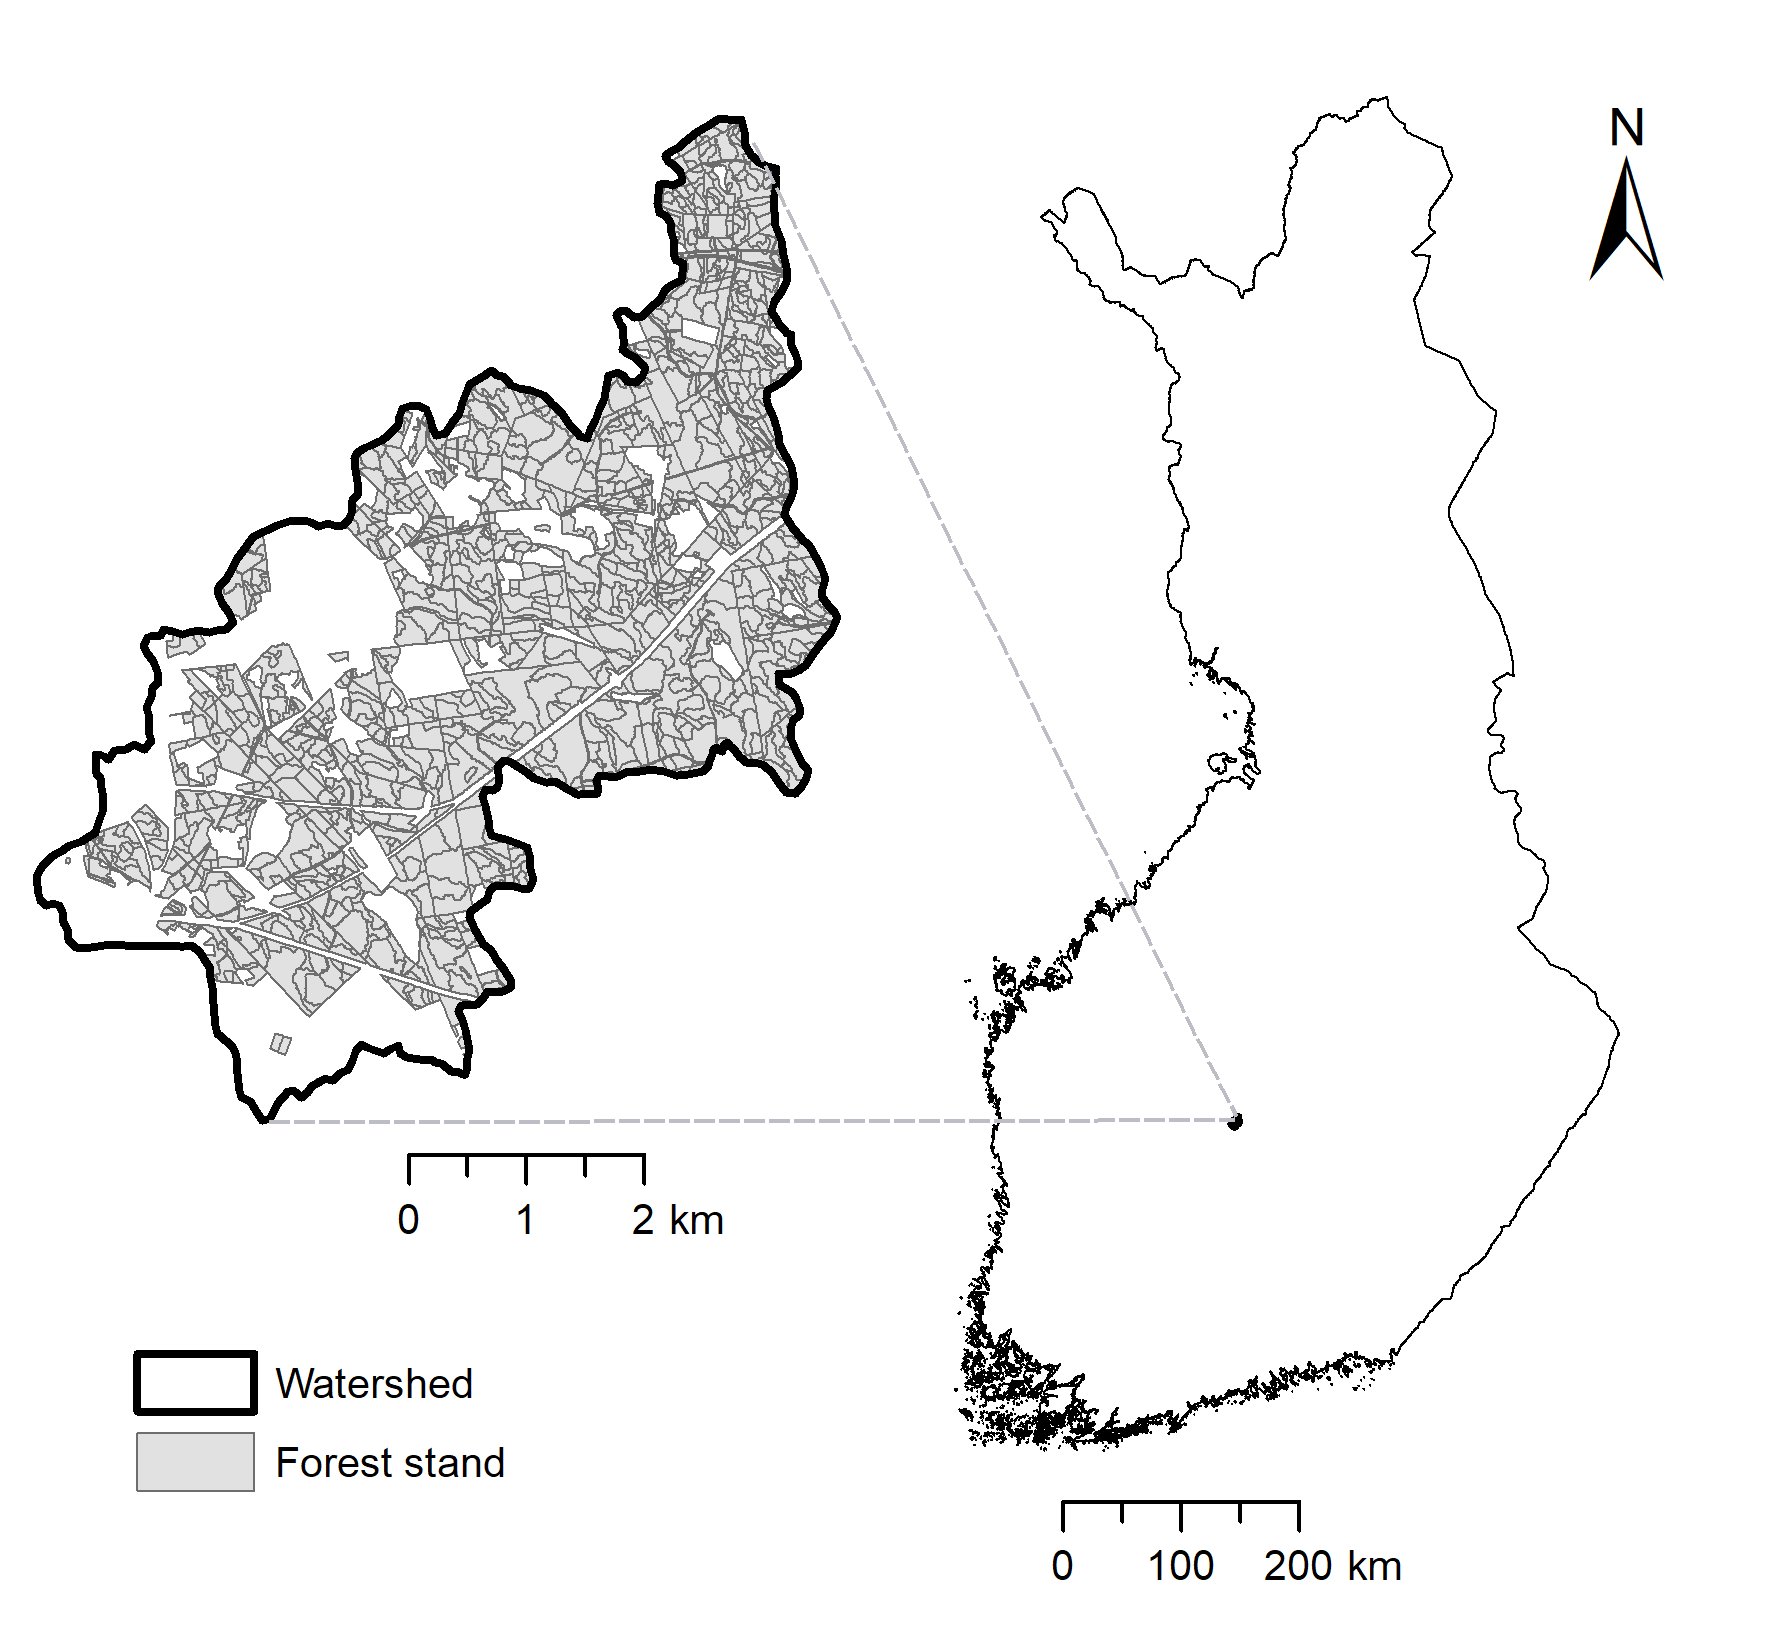
\includegraphics{/projappl/project_2003256/windDamage/externalFigs/studyArea_crop.png}
\caption{The study area located in Central Finland (watershed 14.534) comprising 1475 forest stands.\label{study_area}}
\end{figure}

Our input dataset includes initial stand conditions (2016), alternative forest growth under the range of forest managemnet regimes over 100 years and a set of optimal solutions balancing between intensifying harvest levels and multifunctionnality (from completely set-aside, i.e.~no management to maximal harvest gains). From the set of optimal solutions we have calculated stand-level probability of wind damage (for full details, please refer to Eyvindson et al. (2021) study. Fig. \ref{workflow}) represents study workflow.

\begin{figure}
\centering
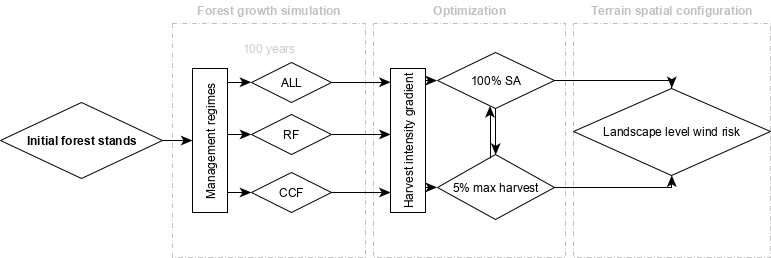
\includegraphics{/projappl/project_2003256/windDamage/externalFigs/overview2_horizontal.png}
\caption{The study workflow from collecting initial stand conditions (2016) throught forest simulation growth under various ranges of forest management, and constriuction of teh harvesting intensity gradient using optimization to landscape level stand configurations.\label{workflow}}
\end{figure}

\hypertarget{forest-stand-development-under-different-regimes}{%
\subsection{Forest stand development under different regimes}\label{forest-stand-development-under-different-regimes}}

We simulated the development of the forests stands using SIMO forest growth simulator (Rasinmäki et al., 2009) over 100 years, separated into 20 5-year sequences. Each stand could be managed by up to 58 different management regimes (the total number of regimes per stands depended on the initial stand conditions), including 17 regimes for rotation forestry (RF), 40 variations of continuous cover forest (CCF) and one set-aside (SA), where no management actions were taken. RF regimes differed in timing of final felling, optional thinning (present/absent), and increase in number of retained green trees after final cut (more details in Eyvindson and Kangas (2018)). Basic CCF management follows rules from Äijälä et al. (2014). To increase the range of CCF managements, we varied two rules defining the timing of harvest: (i) site-specific basal area and (ii) timing of the first thinning. We modified the pre-defined site-specific basal area requirement (16m2/ha for less fertile sites to 22m2/ha for fertile sites) prior to harvesting by -3, ±0, +3, +6, and delayed the timing of the first harvest in 5 year increments up to a delay of 45 years.

\hypertarget{optimization}{%
\subsection{Optimization}\label{optimization}}

The optimal forest management explores the trade-offs between net present income (NPI) and forest multifunctionality. NPI represents economic value of the forests estimated by Metsähallitus (the Finnish governmental organization managing state owned forests). Higher NPI presents higher timber extraction and opposes the proportion of the set-aside forest stands (i.e.~without active harvesting) over the landscape. Optimization process over the NPI gradient was run using only RF, only CCF management types, or all possible managements (RF and CCF, further reffered as ALL) included over the gradient of NPI values, from 0 (representing completely set-aside or no management in all stands) to maximal amount of extracted timber (leaving up to 5\% of SA stands). The optimization balances between harvest intensity and landscape-level multifunctionnality, including non-woody ecosystem services (climate change mitigation), recreational activities and vertebrate and non-vertebrate endangered species. The optimization resulted in 63 alternative collections of RF, CCF and ALL manamement regimes. We converted the optimal solutions back to the development paths for every stand under alternative management given group of management allowed (CCF, RF, ALL) and levels of timber extraction (21). Each stand has only one management regime by scenario. This allowed to reconstruct stand structure on particular stand under given management regime at specific time.

\hypertarget{wind-risk-calculation}{%
\subsection{Wind risk calculation}\label{wind-risk-calculation}}

We have calculated the probability of wind damage based on Suvanto et al. (2019) binomial generalized linear model with logit-link function for each stand for every time step at each scenario. Suvanto et al. (2019) model calculates the probability of the wind damage considering available relevant open-access datasets including dominant tree species, dominant tree height, time since thinning, predicted levels on maximal wind speed, temperature sums, evaluated if stand has open edge, soil type, mineral soil depth, site fertility and temperature sum (see Suvanto et al. (2019) for all details). The final probability of wind damage shows relative differences between stands, whereas the damage can be only partial to the stand, but neglects the explicit spatial locations of the future strongs winds. The parameters of the dominant tree species, tree height, open edge and time since thinning were dynamics under simulated management regimes. Parameters of maximal predicted wind speed and temperature sums, as well as soil characteristics, remained stable during our 100 years simulation. We processed the datasets, calculated damage probability models, and visualized results using R Development Core Team (2019).

\hypertarget{data-processing}{%
\subsection{Data processing}\label{data-processing}}

We calculated the probability of wind damage for each stand, scenario and time intervals. Further, we averaged the wind risk values over the scenarios to allow comparison between RF, CCF and ALL management regimes groups over the harvesting gradient. We explored the mean wind risk (\%) given the management groups and over harvest gradient (from set-aside to maximal harvest levels). In addition, we investigated the mean levels of the standing log and pulp timber volumes (m3) for scenarios, and total sum of harvested pulp and log timber over simulation run (XXX). We further investigated the changes in dynamics parameters (tree species, dominant tree height, frequency of open edges and time since thinning) over the harvest intensity gradient to understand how they contributed to predicted wind risk values. As different tree species varied in wind risk probability, we further groupped this variable by species to understand differences between species, Specifically, we calculated mean proportion of individual tree species (\%), mean tree heights (m), proportion of the stands with open edge from total amount of stands by species and mean thinning frequencies by year.

\hypertarget{results}{%
\section{Results}\label{results}}

\hypertarget{how-does-the-proportion-of-the-sa}{%
\section{How does the proportion of the SA}\label{how-does-the-proportion-of-the-sa}}

Get sum of the wind risk in SA/no SA stands over scenarios
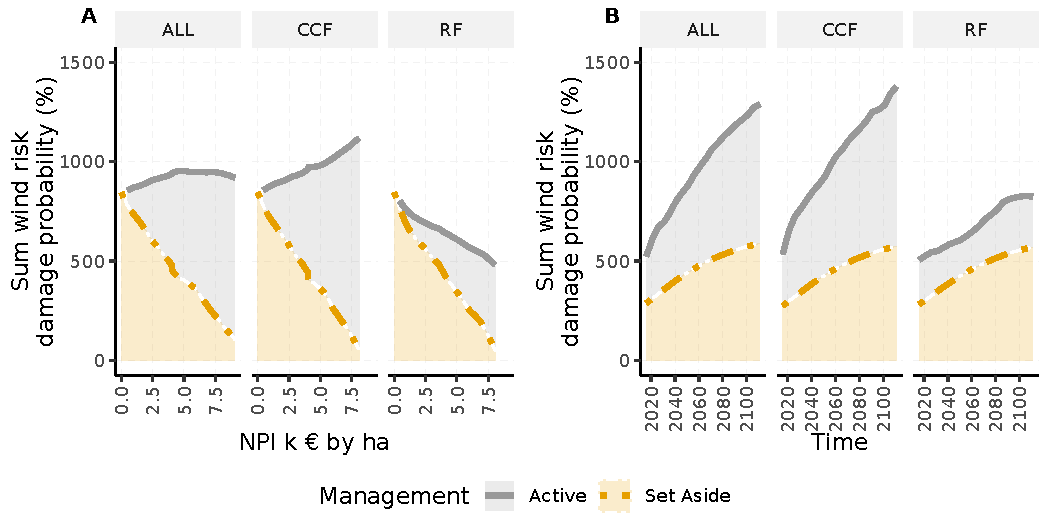
\includegraphics{test_manus3_files/figure-latex/unnamed-chunk-1-1.pdf}

\hypertarget{timber-at-risk-among-scenarios-and-time}{%
\subsection{Timber at risk among scenarios and time}\label{timber-at-risk-among-scenarios-and-time}}

\hypertarget{wind-damage-probability}{%
\subsection{Wind damage probability}\label{wind-damage-probability}}

The level of wind risk remain the same with increasing harvest intensity, while it is two time higher in CCF then in RF (Fig.3). In set-aside stands is stabel until 5K EUR by ha, while afterwards increases. This might be because of the selection of the less profitalne stands as set-aside forests while increasing timber profits. Over time, the probability of wind risk increases in CCF and RF management and culminates towards the end of the simulation period, and in RF it sharply decreases (FIG). the wind risdk in ciompletely set-aside forests almost double over time. @ref\{fig\_meanRisk\_time\_NPI\}

\hypertarget{timber-volume-at-wind-risk}{%
\subsubsection{Timber volume at wind risk}\label{timber-volume-at-wind-risk}}

All three types of management groups responds similarly to set-aside stands: stading timber volume decreases in set-aside stands, which corresponds to preferential selection of the low quality stands to be set as set-aside at the beginning of teh simulation period. Standing mean log timber volume slightly increases with harvesting intensity where increases from 50m3 to 75m3 with the highest increase in RF. In set aside stands, the highest mean top stratum timber volume starts as 150 m3 and lowers to 50 m3/ha with increasing harvest intensity. In pulp wood,RF has three times higher pulp volume compared to CCF as low harvest intensities, the pulp volume in CCF remains relatively stable with increasing harvest intensity.

All three types of management groups responds similarly to set-aside stands: stading timber volume decreases in set-aside stands, which corresponds to preferential selection of the low quality stands to be set as set-aside at the beginning of teh simulation period. Standing mean log timber volume slightly increases with harvesting intensity where increases from 50m3 to 75m3 with the highest increase in RF. In set aside stands, the highest mean top stratum timber volume starts as 150 m3 and lowers to 50 m3/ha with increasing harvest intensity. In pulp wood,RF has three times higher pulp volume compared to CCF as low harvest intensities, the pulp volume in CCF remains relatively stable with increasing harvest intensity. Over time, the log volume culminates in RF in year 2100 to up to 150 m3 in to top layers, while remaines halved in CCF, whereas the pulp volume starts at the same levels for CCF and RF in 2016 and in next 40 years (from 2060) in RF dominates the proportion of teh pulp wood over the CCF. Overall, the log timber in in SA stands increases over time, as they were not logged, and sligtthly decreases in teh amount of pulp wood.

The intensification of the harvesting levels increases the proportion of the pulp wood compared to log wood, especially in RF. In CCF, the proportion among standing log and pulp volume remains at the same rate (65:30) where the production of the log timber dominates. At the highest intensity of timber extraction, pulp wood creates up to 50\% of teh total standing volume See figure @ref(fig:proportion\_V\_pulp\_log) NEW FIG @ref(proportion\_V\_pulp\_log).

In spruce dominated forests, the proportion of the log wood from top stratum lowers by 50\% with increasing harvesting rate in all management regimes applied. Interestingly, RF maintains the high production of the pulp wood with increasing harvest intensity. For all species, the proportion of the stand and top stratum volumes lowers by 47\% (spruce, RF), while pulp lowers in CCF and ALL management (41) and remained the same (mean 100 m3/ha)in RF with increasing harvesting rates.

\begin{figure}
\centering
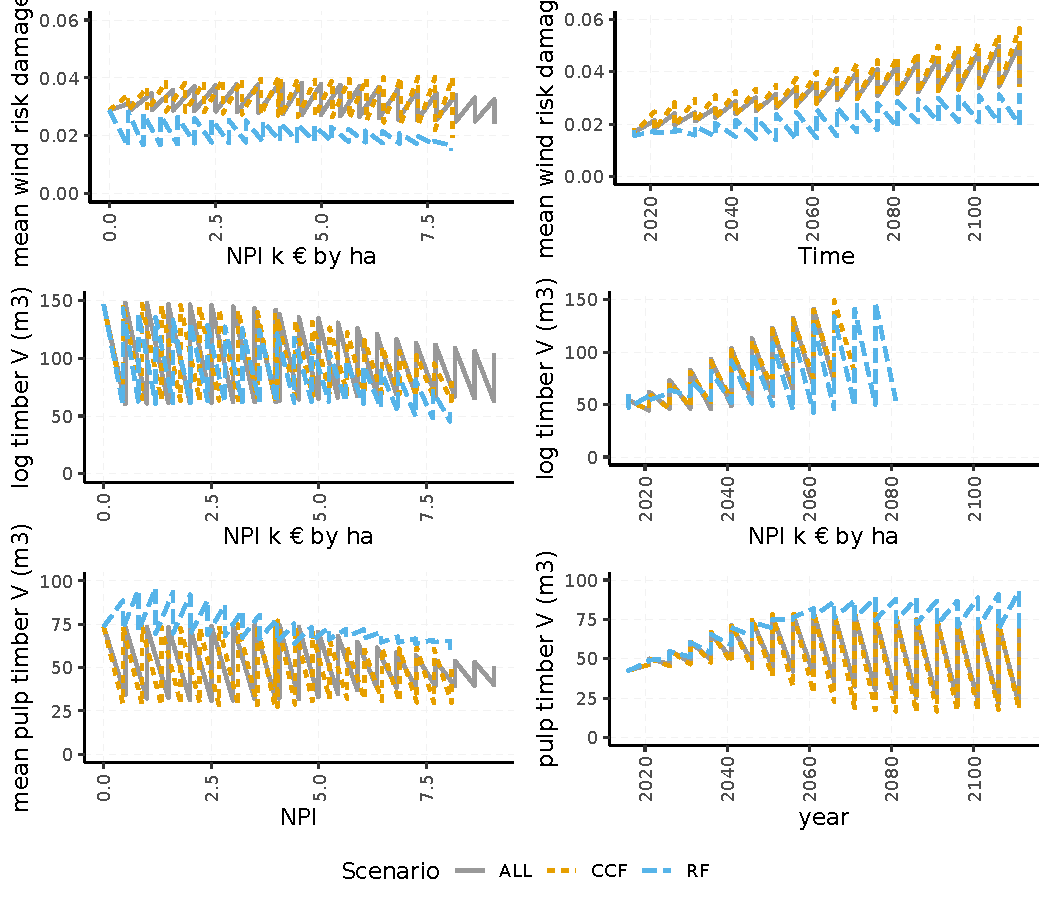
\includegraphics{test_manus3_files/figure-latex/show-plot-volume-1.pdf}
\caption{\label{fig:show-plot-volume}Mean log (left) and pulp (right) timber volume of the top tree layer in the stands over management groups over harvesting intensity gradient (top) and over years (bottom)}
\end{figure}

\hypertarget{dynamic-parameters-contributing-to-wind-risk}{%
\subsection{Dynamic parameters contributing to wind risk}\label{dynamic-parameters-contributing-to-wind-risk}}

\hypertarget{species-composition}{%
\subsubsection{Species composition}\label{species-composition}}

The intensification of the harvesting changes the stand species composition over time (Fig. \ref{species_change}). Intensification of the harvesting favorize the proportion of the Norway spruce and others (deciduous) tree species instead of Scots pine, which likely in turn increases wind risk over the stands. Proportion of the pine lowers with higher harvest intensities.

\hypertarget{dominant-tree-heights}{%
\subsubsection{Dominant tree heights}\label{dominant-tree-heights}}

The intensification of the harvest reduce mean tree height for other species to half (from 20 m to 10 m) in RF, while CCF slightly increases mean tree heights.For pine and spruce trees, harvest intensification maintain the mean tree height of the stand to 20 m(other) to 22 m (spruce). Spruce is higher then pine and other stree species.

\hypertarget{tree-count}{%
\subsubsection{Tree count}\label{tree-count}}

\hypertarget{frequency-of-open-stands}{%
\subsubsection{Frequency of open stands}\label{frequency-of-open-stands}}

The proportion of the open edge stands remains very high over whole simulation run, which is likely due to the fragmeneted landscape (85-95\% of stands by species, Fig. 2, Fig. XX). However, increasing harvest intensity lowers number of stands with open edge when dominated by other species, whereas increases those numbers for pine and spruce dominated spatnd, especially under RF. The CCF and ALL management groups maintain the number of the open edge stands similar to completely set aside stands.

\hypertarget{thinning-frequency}{%
\subsubsection{Thinning frequency}\label{thinning-frequency}}

the highest frequency of thinnings is under CCF management regimes, which lineraly increase with harvesting intensity for all tree species. Numbers of thinnings in RF remains relatively low comparing to CCF and ALL, and strongly increases at high harvest intensity (from 3K for pine and from 5K for spruce). The frequency of thinnings in CCF increases 3-4 times in CCF comparing to RF.

\begin{figure}
\centering
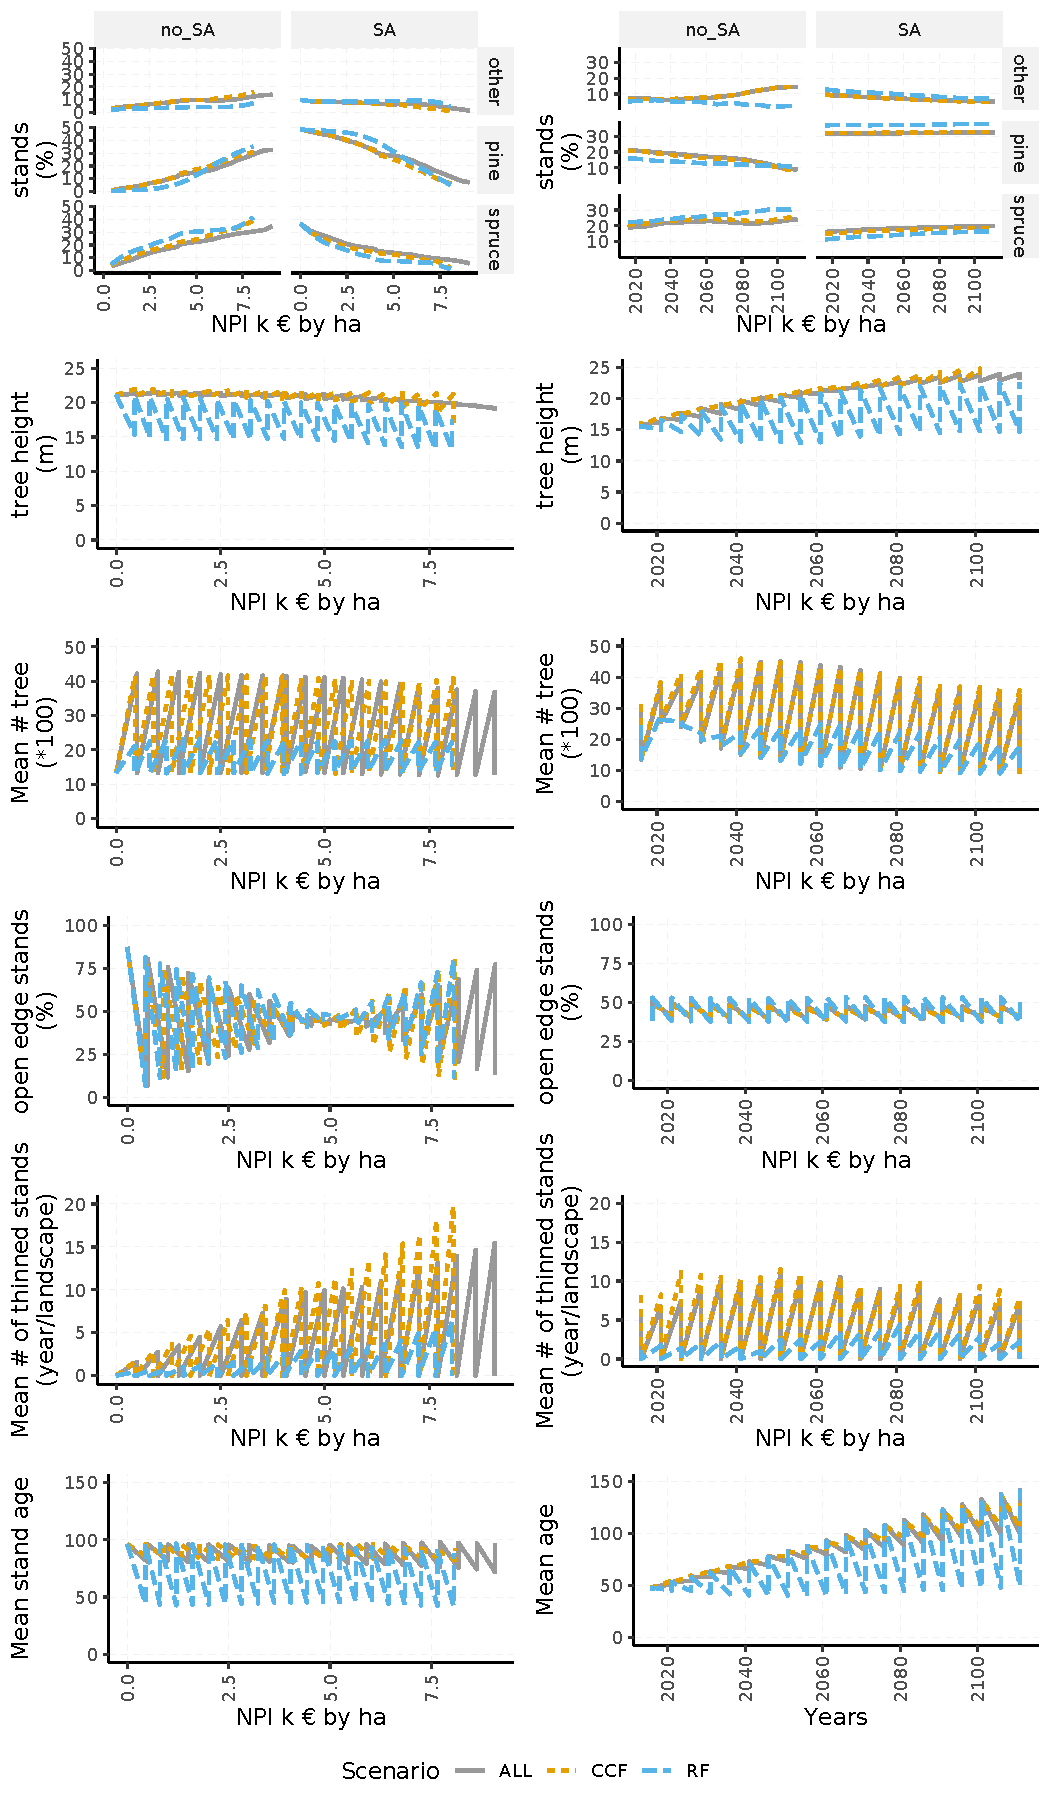
\includegraphics{test_manus3_files/figure-latex/plot-dynamic-vars-1.pdf}
\caption{\label{fig:plot-dynamic-vars}dynamics variables over harvest gradient and years}
\end{figure}

\hypertarget{discussion}{%
\section{Discussion}\label{discussion}}

\hypertarget{wind-risk-dynamics}{%
\subsubsection{Wind risk dynamics}\label{wind-risk-dynamics}}

We found that intensification of the harvesting regimes have different conseuqences of resulting wind risk: where CCF management increases wind risk, and RF lowers wind risk with increasing intensity.

\hypertarget{wind-risk-drivers}{%
\subsubsection{Wind risk drivers}\label{wind-risk-drivers}}

\hypertarget{future-questions-to-answer}{%
\subsubsection{Future questions to answer}\label{future-questions-to-answer}}

\hypertarget{recommendation-for-future-management}{%
\subsubsection{Recommendation for future management}\label{recommendation-for-future-management}}

\begin{itemize}
\tightlist
\item
  SA vs.~intensification of management
\item
  management types: CCF, RF or ALL or something else???
\end{itemize}

Wind (10 years return level of max wind speed REF) are estimated the same over 100 years as well as temperature sums. How does could affects the results?

In spite of inherent stochasticity of the wind and damage phenomena at all spatial scales can be successfully modelled combining spatial spatial datasets and ground earth observation data (Suvanto et al.~2019).
Interpret Suvanto's map: there are 3 limitations:
use values as relative to each other - instead of exact probability valuesm, interpret the map as relative differences in damage vulnerability
Damage probabilities do not refer to complete damage of the stand -- damage can be only poartial, in some part of the stand (not spatially expicit)
map erepresent the forest vulnerability to the wind, but it is impossible to predict the exact locations of future wind disturbances, given uncertainities in future wind occurences

\begin{itemize}
\item
  the glm takes into account the dominant tree species but neglects the stand structure. WE neglected the stand structure in applying the raster level based glm model to stand level information
\item
  difficult to link the predicted wind risk to explicit wind damage volume as windthrows are unpredictanvle events in time and explicit locations.
\item
  We need to understand what risks about current management decisions involves and if they bring another challenges, such as increasing risk of wind damage. On the other hand, the set-aside stands, if protected, teh wind damage there should not be regarded as lost timber volume due to windthrow, as was not supposed to be logged anyway. Howvere, if windthrow happen in SA stands, the risk of subsequent disturbances such as \emph{Ips typographus} might increase the cost of the effective stand protection in following years.
\item
  SA forests have clearly higher wind risk than intensively managemed forests under RF. However, RF as highly specialized in provision of teh single benefit - timber - while deterioration non-woody ecosystem servoices and destroyng habitats for endangered species should be largely replaced over the landscapes by managements fulfillings multiple benefits Eyvindson et al. (2021).
\item
\end{itemize}

The shortening of the rotation period in Norway spruce forets might slightly lower the wind and subsequent bark beetle distudrabnces but has limited efficiencies and decreses under climate change (Zimová et al., 2020)

\hypertarget{conclusion}{%
\section{Conclusion}\label{conclusion}}

\newpage

\hypertarget{references}{%
\section*{References}\label{references}}
\addcontentsline{toc}{section}{References}

\hypertarget{refs}{}
\leavevmode\hypertarget{ref-Aijala2014a}{}%
Äijälä, O., Koistinen, A., Sved, J., Vanhatalo, K., Väisänen, P., 2014. Metsänhoidon suositukset {[}Good forest management recommendations{]}. Forestry Development Center Tapio.

\leavevmode\hypertarget{ref-Eyvindson2021}{}%
Eyvindson, K., Duflot, R., Triviño, M., Blattert, C., Potterf, M., Mönkkönen, M., 2021. High boreal forest multifunctionality requires continuous cover forestry as a dominant management. Land Use Policy 100, 1--10. doi:\href{https://doi.org/10.1016/j.landusepol.2020.104918}{10.1016/j.landusepol.2020.104918}

\leavevmode\hypertarget{ref-Eyvindson2018}{}%
Eyvindson, K., Kangas, A., 2018. Guidelines for risk management in forest planning --- what is risk and when is risk management useful? Canadian Journal of Forest Research 48, 309--316. doi:\href{https://doi.org/10.1139/cjfr-2017-0251}{10.1139/cjfr-2017-0251}

\leavevmode\hypertarget{ref-Peura2018}{}%
Peura, M., Burgas, D., Eyvindson, K., Repo, A., Mönkkönen, M., 2018. Continuous cover forestry is a cost-efficient tool to increase multifunctionality of boreal production forests in Fennoscandia. Biological Conservation 217, 104--112. doi:\href{https://doi.org/10.1016/j.biocon.2017.10.018}{10.1016/j.biocon.2017.10.018}

\leavevmode\hypertarget{ref-Pohjanmies2019}{}%
Pohjanmies, T., Eyvindson, K., Mönkkönen, M., 2019. Forest management optimization across spatial scales to reconcile economic and conservation objectives. PLoS ONE 14, 1--16. doi:\href{https://doi.org/10.1371/journal.pone.0218213}{10.1371/journal.pone.0218213}

\leavevmode\hypertarget{ref-Rasinmaki2009}{}%
Rasinmäki, J., Mäkinen, A., Kalliovirta, J., 2009. SIMO: An adaptable simulation framework for multiscale forest resource data. Computers and Electronics in Agriculture 66, 76--84. doi:\href{https://doi.org/10.1016/j.compag.2008.12.007}{10.1016/j.compag.2008.12.007}

\leavevmode\hypertarget{ref-RDevelopmentCoreTeam2019}{}%
R Development Core Team, 2019. R: A language and environment for statistical computing.

\leavevmode\hypertarget{ref-Suvanto2019}{}%
Suvanto, S., Peltoniemi, M., Tuominen, S., Strandström, M., Lehtonen, A., 2019. High-resolution mapping of forest vulnerability to wind for disturbance-aware forestry. Forest Ecology and Management 453, 117619. doi:\href{https://doi.org/10.1016/j.foreco.2019.117619}{10.1016/j.foreco.2019.117619}

\leavevmode\hypertarget{ref-Trivino2017}{}%
Triviño, M., Pohjanmies, T., Mazziotta, A., Juutinen, A., Podkopaev, D., Le Tortorec, E., Mönkkönen, M., 2017. Optimizing management to enhance multifunctionality in a boreal forest landscape. Journal of Applied Ecology 54. doi:\href{https://doi.org/10.1111/1365-2664.12790}{10.1111/1365-2664.12790}

\leavevmode\hypertarget{ref-Zimova2020}{}%
Zimová, S., Dobor, L., Hlásny, T., Rammer, W., Seidl, R., 2020. Reducing rotation age to address increasing disturbances in Central Europe : Potential and limitations. Forest Ecology and Management 1--50.


\end{document}


